%%%%%%%%%%%%%%%%%%%%%%%%%%%%%%%%%%%%%%%%%%%%%%%%%%%%%%%%%%%%%%%%%%%%%%%%%%%%%%%%%
%																				%
%	TRABAJO:	Trabajo Final													%
%				Especialidad en Ingenier�a en Sistemas de Informaci�n			%
%																				%
%		Titulo:																	%
%																				%
%		Autores:	Julian Nonino												%
%																				%
%	Capitulo sobre Docker														%	
%																				%
%	A�o: 2016																	%
%																				%
%%%%%%%%%%%%%%%%%%%%%%%%%%%%%%%%%%%%%%%%%%%%%%%%%%%%%%%%%%%%%%%%%%%%%%%%%%%%%%%%%

\chapter{Docker}

Docker es un proyecto de c�digo abierto que automatiza el despliegue de
aplicaciones dentro de contenedores de software, proporcionando una capa
adicional de abstracci�n y automatizaci�n de virtualizaci�n a nivel de sistema
operativo en Linux. Docker utiliza caracter�sticas de aislamiento de recursos
del kernel de Linux, tales como cgroups y espacios de nombres (namespaces) para
permitir que \emph{contenedores} independientes se ejecuten dentro de una sola
instancia de Linux, evitando la sobrecarga de iniciar y mantener m�quinas
virtuales. \cite{WikipediaDocker}

El soporte del kernel de Linux para los espacios de nombres a�sla de vista, en
su mayor�a, una aplicaci�n del entorno operativo, incluyendo �rboles de proceso,
red, ID de usuario y sistemas de archivos montados, mientras que los cgroups del
kernel proporcionan aislamiento de recursos, incluyendo la CPU, la memoria, el
bloque de E/S y de la red. Desde la versi�n 0.9, Docker incluye la librer�a
libcontainer como su propia manera de utilizar directamente las facilidades de
virtualizaci�n que ofrece el kernel de Linux, adem�s de utilizar las interfaces
abstra�das de virtualizaci�n mediante libvirt, LXC (Linux Containers) y
systemd-nspawn. \cite{WikipediaDocker}

Docker implementa una API de alto nivel para proporcionar contenedores livianos
que ejecutan procesos de manera aislada.
Construido sobre las facilidades proporcionadas por el kernel de Linux
(principalmente cgroups y namespaces), un contenedor Docker, a diferencia de una
m�quina virtual, no requiere incluir un sistema operativo independiente. En su
lugar, se basa en las funcionalidades del kernel y utiliza el aislamiento de
recursos (CPU, la memoria, el bloque E/S, red, etc.) y namespaces separados
para aislar de vista la aplicaci�n del sistema operativo. Docker accede a la
virtualizaci�n del kernel de Linux ya sea directamente a trav�s de la biblioteca
libcontainer (disponible desde Docker 0.9), o indirectamente a trav�s de
libvirt, LXC o systemd-nspawn. \cite{WikipediaDocker}

\begin{figure}[H]
	\centering
	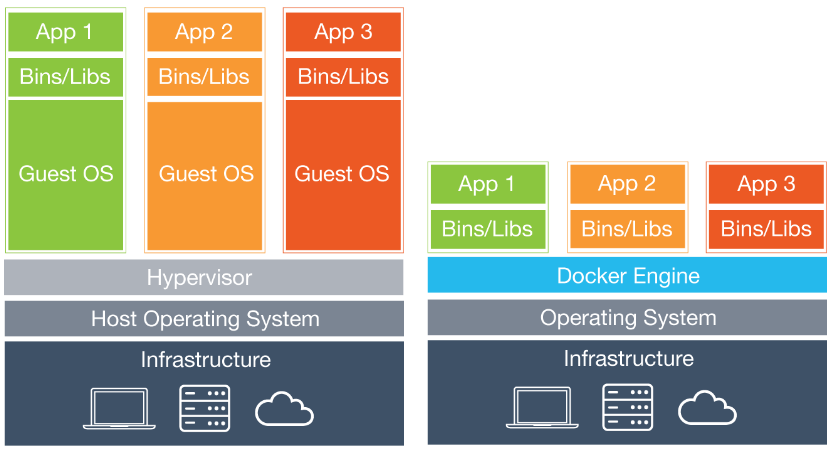
\includegraphics[width=1\linewidth]{./marco_teorico/img/vm-vs-docker}
	\caption{Contenedor Docker (derecha) versus M�quina Virtual (izquierda)
	\cite{WhatIsDocker2016}}
\end{figure}

Mediante el uso de contenedores, los recursos pueden ser aislados, los servicios
restringidos, y se otorga a los procesos la capacidad de tener una visi�n casi
completamente privada del sistema operativo con su propio identificador de
espacio de proceso, la estructura del sistema de archivos, y las interfaces de
red. Contenedores m�ltiples comparten el mismo n�cleo, pero cada contenedor
puede ser restringido a utilizar s�lo una cantidad definida de recursos como
CPU, memoria y E/S. \cite{WikipediaDocker}

Usando Docker para crear y gestionar contenedores puede simplificar la creaci�n
de sistemas altamente distribuidos, permitiendo m�ltiples aplicaciones, las
tareas de los trabajadores y otros procesos para funcionar de forma aut�noma en
una �nica m�quina f�sica o en varias m�quinas virtuales. Esto permite que el
despliegue de nodos se realice a medida que se dispone de recursos o cuando se
necesiten m�s nodos, lo que permite una plataforma como servicio (PaaS -
Plataform as a Service) de estilo de despliegue y ampliaci�n de los sistemas
como Apache Cassandra, MongoDB o Riak. Docker tambi�n simplifica la creaci�n y
el funcionamiento de las tareas de carga de trabajo o las colas y otros sistemas
distribuidos. \cite{WikipediaDocker}

\section{Imagenes y Contenedores}



\section{Docker Compose}

	Docker Compose es una herramienta que permite correr un sistema formado por
	m�ltiples contenedores.
	
	
